%%%%%%%%%%%%%%%%%%%%%%%%%%%%%%%%%%%%%%%%%
% Short Sectioned Assignment
% LaTeX Template
% Version 1.0 (5/5/12)
%
% This template has been downloaded from:
% http://www.LaTeXTemplates.com
%
% Original author:
% Frits Wenneker (http://www.howtotex.com)
%
% License:
% CC BY-NC-SA 3.0 (http://creativecommons.org/licenses/by-nc-sa/3.0/)
%
%%%%%%%%%%%%%%%%%%%%%%%%%%%%%%%%%%%%%%%%%

%----------------------------------------------------------------------------------------
%       PACKAGES AND OTHER DOCUMENT CONFIGURATIONS
%----------------------------------------------------------------------------------------

\documentclass[paper=a4, fontsize=11pt]{scrartcl} % A4 paper and 11pt font size

\usepackage[T1]{fontenc} % Use 8-bit encoding that has 256 glyphs
%\usepackage{fourier} % Use the Adobe Utopia font for the document - comment this line to return to the LaTeX default
\usepackage[english]{babel} % English language/hyphenation
\usepackage{amsmath,amsfonts,amsthm} % Math packages
\usepackage{graphicx}
\usepackage{listings}
\usepackage{color}
\usepackage{float}
\usepackage[top=1.5in, bottom=1.5in, left=1in, right=1in]{geometry}
\usepackage{setspace}
\usepackage{lipsum} % Used for inserting dummy 'Lorem ipsum' text into the template
\usepackage{framed}
\usepackage{hyperref}
\usepackage[ruled]{algorithm2e}
\usepackage{sectsty} % Allows customizing section commands
\allsectionsfont{\normalfont\scshape} % Make all sections centered, the default font and small caps

\usepackage{fancyhdr} % Custom headers and footers
%\pagestyle{empty} % Makes all pages in the document conform to the custom headers and footers

\renewcommand{\headrulewidth}{0pt} % Remove header underlines
\renewcommand{\footrulewidth}{0pt} % Remove footer underlines
\setlength{\headheight}{13.6pt} % Customize the height of the header

%\numberwithin{equation}{section} % Number equations within sections (i.e. 1.1, 1.2, 2.1, 2.2 instead of 1, 2, 3, 4)
%\numberwithin{figure}{section} % Number figures within sections (i.e. 1.1, 1.2, 2.1, 2.2 instead of 1, 2, 3, 4)
%\numberwithin{table}{section} % Number tables within sections (i.e. 1.1, 1.2, 2.1, 2.2 instead of 1, 2, 3, 4)

%\setlength\parindent{0pt} % Removes all indentation from paragraphs - comment this line for an assignment with lots of text


\definecolor{mygreen}{rgb}{0,0.6,0}
\definecolor{mygray}{rgb}{0.5,0.5,0.5}
\definecolor{mymauve}{rgb}{0.58,0,0.82}

\lstset{ %
  backgroundcolor=\color{white},   % choose the background color; you must add \usepackage{color} or \usepackage{xcolor}
  basicstyle=\scriptsize,        % the size of the fonts that are used for the code
  breakatwhitespace=false,         % sets if automatic breaks should only happen at whitespace
  breaklines=true,                 % sets automatic line breaking
  captionpos=b,                    % sets the caption-position to bottom
  commentstyle=\color{mygreen},    % comment style
  deletekeywords={...},            % if you want to delete keywords from the given language
  escapeinside={\%*}{*)},          % if you want to add LaTeX within your code
  extendedchars=true,              % lets you use non-ASCII characters; for 8-bits encodings only, does not work with UTF-8
  frame=single,                    % adds a frame around the code
  keepspaces=true,                 % keeps spaces in text, useful for keeping indentation of code (possibly needs columns=flexible)
  keywordstyle=\color{mygreen},       % keyword style
  language=matlab,                 % the language of the code
  morekeywords={vector,...},            % if you want to add more keywords to the set
  numbers=left,                    % where to put the line-numbers;
                                % possible values are (none, left,
                                % right)
  identifierstyle=\color{blue},
  numbersep=5pt,                   % how far the line-numbers are from the code
  numberstyle=\tiny \color{mygray} , % the style that is used for the line-numbers
  rulecolor=\color{black},         % if not set, the frame-color may be changed on line-breaks within not-black text (e.g. comments (green here))
  showspaces=false,                % show spaces everywhere adding particular underscores; it overrides 'showstringspaces'
  showstringspaces=false,          % underline spaces within strings only
  showtabs=false,                  % show tabs within strings adding particular underscores
  stepnumber=2,                    % the step between two line-numbers. If it's 1, each line will be numbered
  stringstyle=\color{mymauve},     % string literal style
  tabsize=2,                       % sets default tabsize to 2 spaces
  title=\lstname                   % show the filename of files included with \lstinputlisting; also try caption instead of title
}


%----------------------------------------------------------------------------------------
%       TITLE SECTION
%----------------------------------------------------------------------------------------

\newcommand{\horrule}[1]{\rule{\linewidth}{#1}} % Create horizontal rule command with 1 argument of height

\title{ 
\normalfont \normalsize 
\textsc{CAAM Rice University} \\ [25pt] % Your university, school and/or department name(s)
\horrule{0.5pt} \\[0.4cm] % Thin top horizontal rule
\huge {CAAM 551: Final Project \\ 
{\Large Spectral Element Method and Additive
  Schwarz Preconditioner}}  \\ % The assignment title
\horrule{2pt} \\[0.5cm] % Thick bottom horizontal rule
}

\author{Zheng Wang} % Your name
\date{}
%\date{\normalsize\today} % Today's date or a custom date
\doublespacing
\begin{document}

\maketitle % Print the title

\section{Problem Description}
In this final project, I want solve the 2D Poisson's equation
\begin{equation}
\left\{
\begin{array}{ll}
-\Delta u = f & \textrm{in } \Omega \\
u = 0 & \textrm{on } \partial \Omega
\end{array}
\right.
\label{poisson}
\end{equation}
where $\Omega = [-1,1]^2$.

This equation has already been solved in many different ways. In this
project, I have applied the spectral element method (SEM) and the
additive Schwarz preconditioner to this problem. 

The purpose is implementing an effective SEM solver and examining the
additive Schwarz preconditioner.

\section{Methods}

This project focuses on two methods: one is the spectral element
method for solving the PDE; the other is the additive Schwarz method
for preconditioning. This section briefly introduces these two methods.

\subsection{Spectral Element Method}

The SEM is a formulation of the finite element method (FEM). The
discretization of the SEM is similar to that of the FEM, and details
of the SEM can be referred to \cite{Dev02}.

To formulate the linear system of the SEM, we multiply a test function
$v$ on both sides of the PDE
(\ref{poisson}), integrate both sides over the domain $\Omega$, and
apply integration by parts. The following equality can be thereby obtained,
\begin{equation}
\int_{\Omega}\nabla u \cdot \nabla v = \int_{\Omega}fv
\end{equation}

Denoting $u$ as the linear combination of basis functions
\begin{equation}
u = \sum_{i} \hat{u}_i \varphi_i
\end{equation}
and letting $v$ run over all the basis functions, we arrive at the
following system,
\begin{equation}
A \hat{u} = b
\label{linsys}
\end{equation}
where $A_{i,j} = \int_{\Omega}\nabla \varphi_i \cdot \nabla \varphi_j$
is the stiffness matrix, $b_i = \int_{\Omega} f \varphi_i$ is the
right-hand side and $\hat{u} = [ \hat{u}_1, \hat{u}_2
  \dots ]$ are the
coefficients of basis functions in the solution.


Different from the FEM, the SEM uses
high degree piecewise polynomials as basis functions. 
In order to make high order polynomials applicable, the SEM employs
rectangular elements and
Gauss-Lobatto-Legendre (GLL) nodes which
enables the Gauss quadrature in the computation. 

Since matrix $A$ in equation (\ref{linsys}) is symmetric positive definite (s.p.d.), the conjugate
gradient (CG) method is suitable for solving the linear system
(\ref{linsys}). 

\begin{figure}[H]
	\centering
        \begin{tabular}{cc}
          \scalebox{0.45}{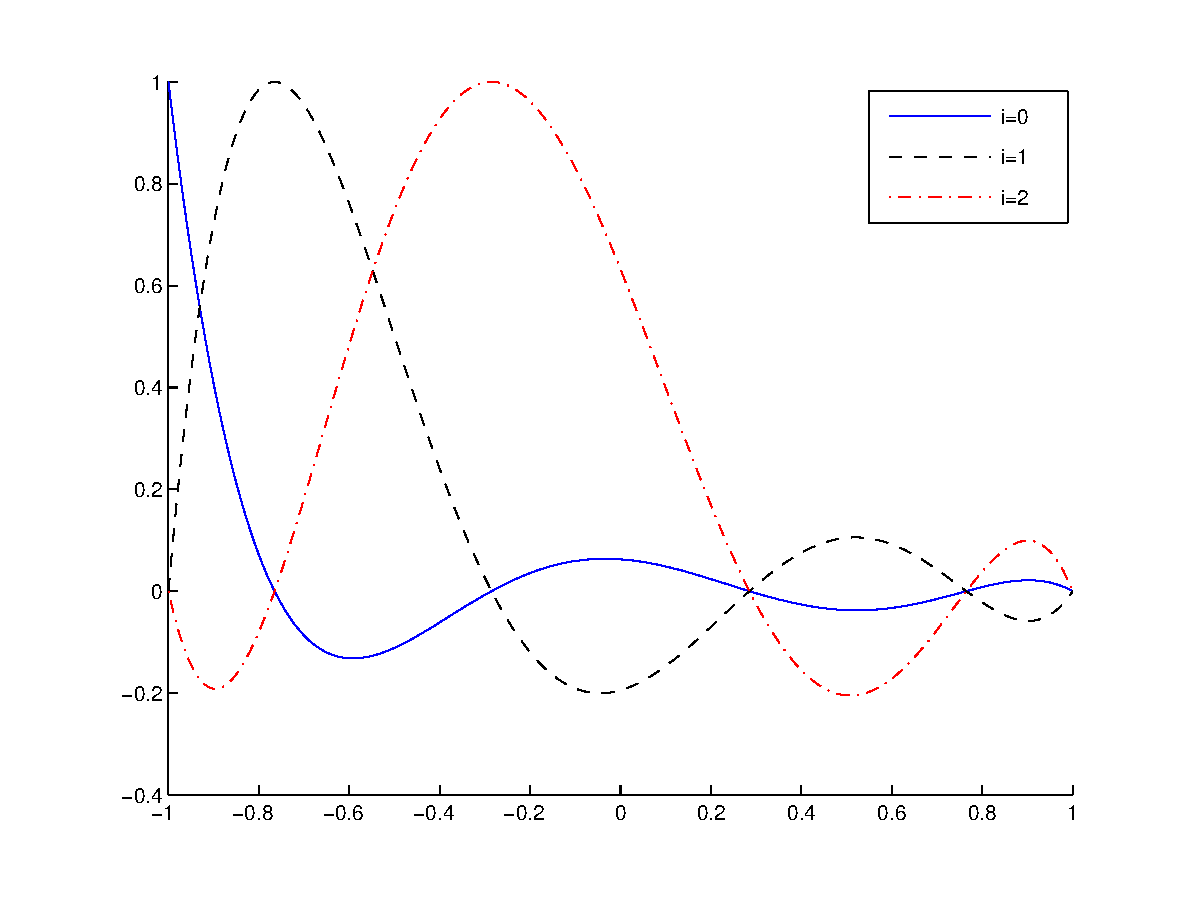
\includegraphics[width=1\textwidth]{Figures/gll1D.eps}} 
          &
          \scalebox{0.45}{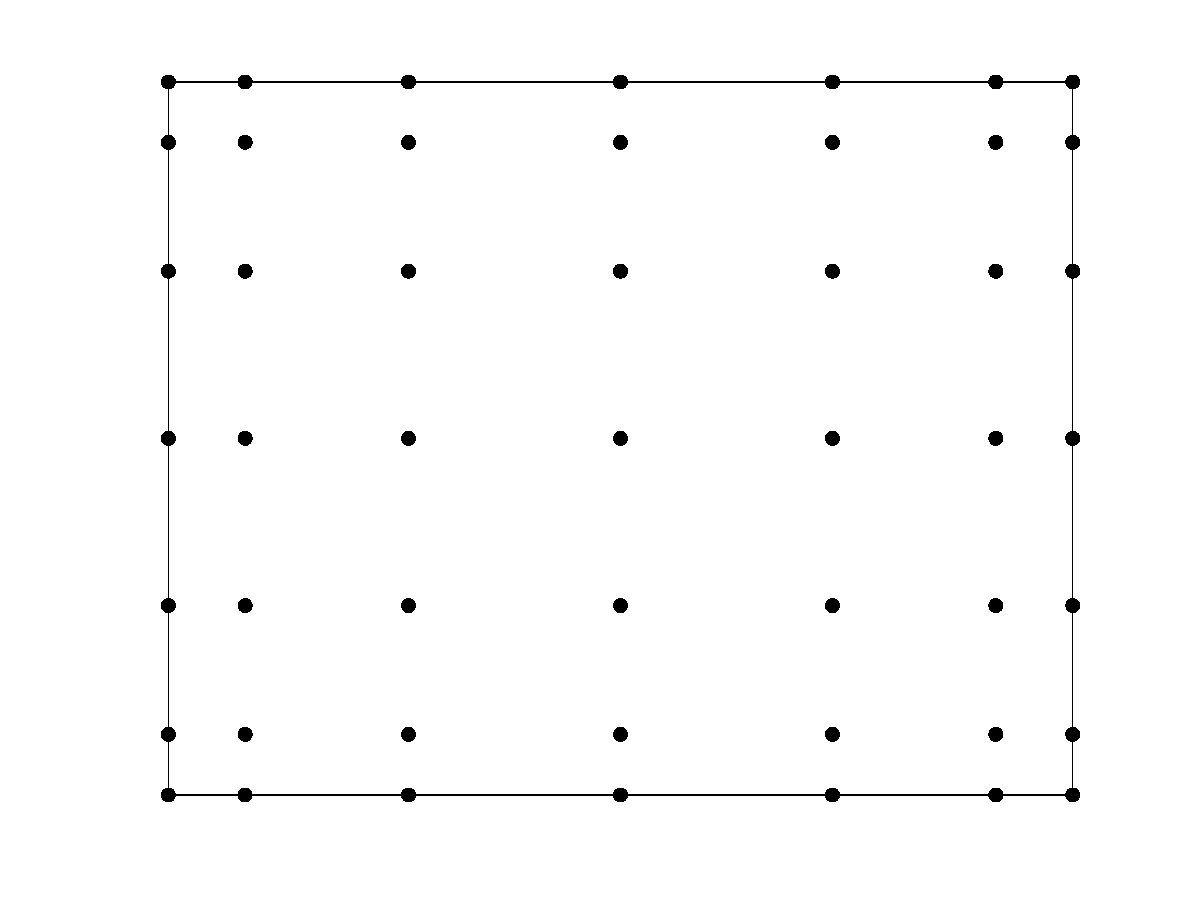
\includegraphics[width=1\textwidth]{Figures/gll2D.eps}}  
          \\
          (a) & (b) \\
        \end{tabular}
        \caption[GLL Nodes]{(a) 1D GLL Interpolation. (b) 2D GLL Nodes}
	\label{GLLNodes}
\end{figure}


However, the condition number of $A$ grows quickly as the polynomial
degree $N$ increases or the mesh sizes $h$ decreases. According to the
literature, the condition number of $A$ is in the scale of
$O(N^4/h^2)$. Because of this fact, a preconditioned conjugate
gradient (PCG) method is a better choice for the SEM solver. 

\subsection{Additive Schwarz Preconditioner}

In the following context, the capital letter $M$
is denoted as the preconditioner matrix and we want to minimize
$\textrm{cond}(M^{-1}A)$ at a low cost. The preconditioner in this
project is the additive Schwarz preconditioner. I read the first
several sections of \cite{chan94} which is a review of domain
decomposition and implemented it to my SEM solver.

Additive Schwarz algorithm is an overlapping subdomain algorithm. To initiate
this algorithm, we need an overlapping decomposition of domain
$\Omega$ into $p$ subregions $\hat{\Omega}_1, \dots, \hat{\Omega}_p$.
To construct this, let ${\Omega}_1, \dots, {\Omega}_p$ be a
nonoverlapping decomposition, where $\Omega_i$ are chosen from a 
 mesh $\tau^h$ of size $h$. Next, we extend $\Omega_i$
to $\hat{\Omega}_i$ by select all the points within a distance of
$\beta h$ from $\Omega_i$, thus
\begin{equation}
\hat{\Omega}_i = \{ x \in \Omega : d(x,\Omega_i) < \beta h\}
\end{equation}
See Figure \ref{overlap} for illustration of a
2D region.

\begin{figure}[h]
	\centering
        \begin{tabular}{ccc}
          \scalebox{0.33}{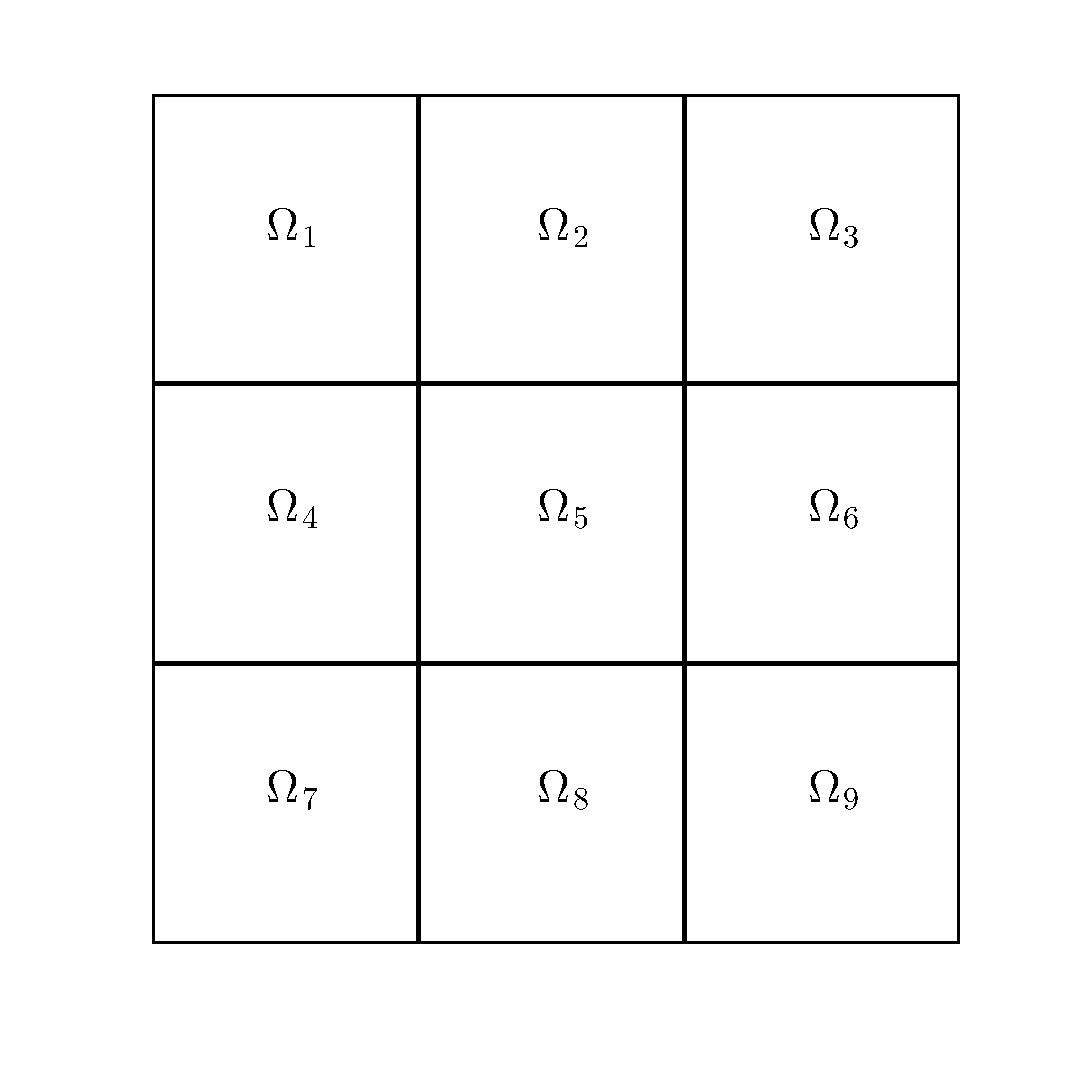
\includegraphics[width=1\textwidth]{Figures/overlap1.eps}} 
          &
          \scalebox{0.33}{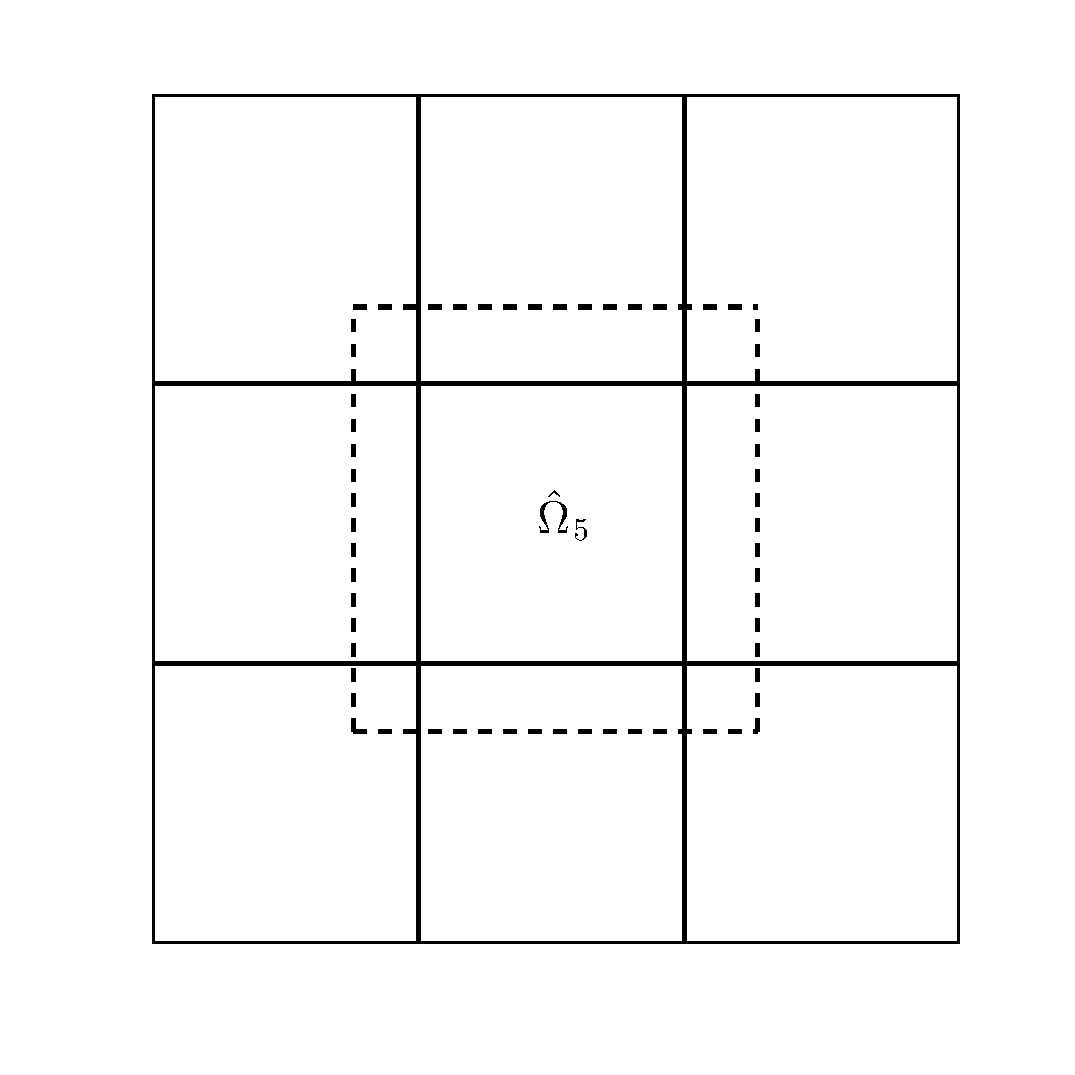
\includegraphics[width=1\textwidth]{Figures/overlap2.eps}} 
          &
          \scalebox{0.33}{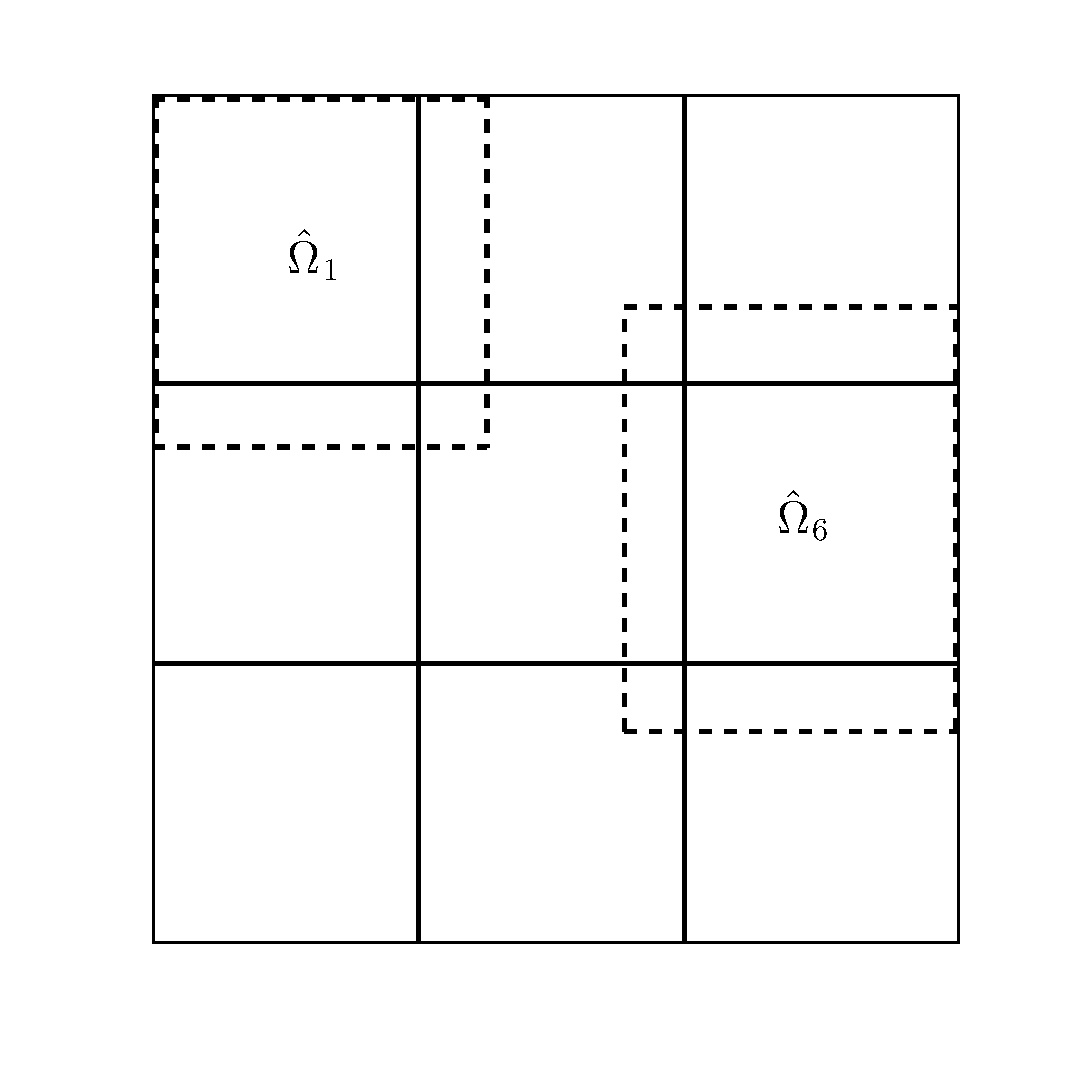
\includegraphics[width=1\textwidth]{Figures/overlap3.eps}} 
          \\
          (a) & (b) & (c)\\
        \end{tabular}
        \caption[Overlapping Subdomain]{(a) Nonoverlapping partition
          (b) Overlapping subdomain: $\hat{\Omega}_5$
        (c) Overlapping subdaomains: $\hat{\Omega}_1$ and  $\hat{\Omega}_6$}
	\label{overlap}
\end{figure}

Once all the $\hat{\Omega}_i$ are well defined, we begin to define
restriction maps $R_i$, extension maps $R_i^T$ and local matrices
$A_i$ corresponding to each subdomain $\hat{\Omega}_i$. Let $A$ be
$n\times n$, $\{ \hat{I}_1, \dots, \hat{I}_p \}$ denote the indices of
the nodes in $\hat{\Omega}_i$, and the cardinality
$|\hat{I}_i| = \hat{n}_i$. For each region $\hat{\Omega}_i$, $R_i$ denotes the
$\hat{n}_i\times n$ restriction matrix. $R_i$ maps a vector $x$ of
length $n$ to a vector
$R_ix$ of length $\hat{n}_i$. If $\hat{I}_i(k)$ is the $k$th element of
$\hat{I}_i$, we can write
\begin{equation}
(R_ix)_k = (x)_{\hat{I}_i(k)}
\end{equation}
$R_i^T$ is the transpose of $R_i$ and it extends a vector
$x_i$ of length $\hat{n}_i$ to a vector $R_i^Tx_i$ of length $n$ by
filling the rest entries which do not have indices in $\hat{I}_i$
with $0$s. We have
\begin{equation}
  (R_i^Tx_i)_k =
  \left\{
    \begin{array}{ll}
      (x_i)_k & \textrm{for} \quad k \in \hat{I}_i \\
      0 & \textrm{for} \quad k \not\in \hat{I}_i
    \end{array}
  \right.
\end{equation}
Finally we let $A_i = R_iAR_i^T$ which is a principal submatrix of $A$
corresponding to subdomain $\hat{\Omega}_i$.

A one-level preconditioner can be then generalized as the following,
\begin{equation}
M_1^{-1}  = \sum_{i=1}^p R_i^T A_i^{-1} R_i
\end{equation}


The overlapping enables one subdomain to have a communication with its
halos. If we pay a small cost to build a global communication of
information for the subdomains, we can do a better job.

To this end, we need an assumption that the fine grid $\tau^h$ is a
refinement of a coarse mesh $\tau^H$. Suppose there are $n_c$ coarse
gird vertices and let $R_0^T$ denote a $n \times n_c$ matrix
which extends coarse gird vertices to the fine grid. Similarly,
 $R_0$ is the transpose of $R_0^T$ and $A_0 = R_0AR_0^T$. the
two-level preconditioner $M_2$ is
\begin{equation}
M_2^{-1} = \sum_{i=0}^pR_i^TA_i^{-1}R_i
\end{equation}

\section{Implementation Details}

This section discusses the implementation details in the project. The
source code can be found at \url{https://github.com/zw14/CAAM551}.

\subsection{SEM Mesh}

In this project, the mesh grid is a structured grid. It is equally
spaced in both dimensions. We set
\begin{equation}
dx = dy = h
\end{equation}
since our domain $\Omega$ is $[-1,1]^2$, each subdomain $\Omega_i$ is
in the form of
\begin{equation}
\Omega_i = [-1+(m-1)\cdot dx, -1+m \cdot dx] \times [-1+(n-1)\cdot dy, -1+n \cdot dy]
\end{equation}

\subsection{Overlapping Region}

In the implementation, the overlapping domain $\hat{\Omega}_i$
extends $\Omega_i$ by one layer of its halo nodes. Hence, the higher
the polynomial degree, the smaller the overlapping region.
\begin{figure}[H]
	\centering
        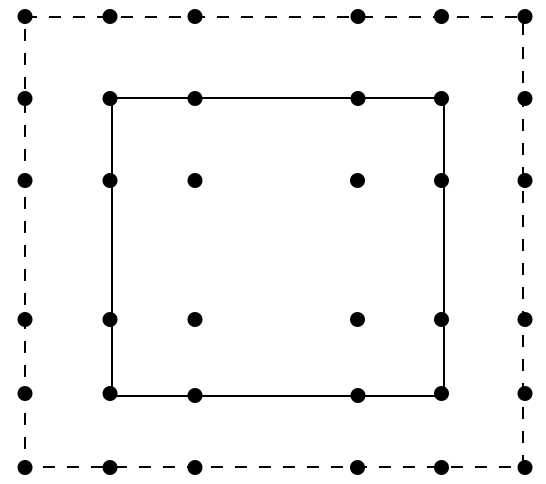
\includegraphics[width=0.3\textwidth]{Figures/lapregion.png}
        \caption[Overlapping Region]{Overlapping Region: the solid
          line square is the non-overlapping element $\Omega_i$, the dash
      line square is the overlapping element $\hat{\Omega}_i$}
	\label{lapregion}
\end{figure}
\subsection{Matrix Free}

In the PCG process, matrix-vector multiplications are
conducted. Instead of storing a matrix, we regard the matrix as an
operator and implement the matrix-vector multiplication without
storing the matrix.

This technic is applied to the stiffness matrix $A$, restriction
matrix $R_i$ and extension matrix $R_i^T$. 

For $A$, we compute the contribution of each element, and scatter the
contribution to the vector. For $R_i$, we collect the entries
of a given vector by a predefined index set. For $R_i^T$, we scatter
the values in a small vector to a large vector.

However, the matrix free technic is not applied to the overlapping
subdomain matrix $A_i$, because $A_i^{-1}$ is required in the PCG process.

\subsection{BLAS \& LAPACK}

To obtain $A_i^{-1}$, BLAS \& LAPACK is used to compute the LU
factorization of $A_i$.  The factorized $A_i$ is computed one time and stored
in the preprocessing part, and hence can be used in the PCG iterations.

\subsection{OpenMP}
Both SEM and additive Schwarz preconditioner are highly
parallelizable. The implementation uses OpenMP to accelerate the
iterations.


\section{Results}
In the test, we choose different mesh sizes $h$ and polynomial order $N$, and
compare the number of iterations and time cost among naive CG,
one-level additive Schwarz and two-level additive Schwarz.



Some basic configurations are:
\begin{itemize}
\item In the two-level additive Schwarz preconditioner, the coarse mesh are
made up of the center nodes in the subdomains in the fine mesh. 
\item The terminating criteria for CG/PCG iterations is that the residue $r$
is less than a tolerance of $1e-3$. 
\item The exact solution used in the test case is
  $u=e^{(x^2-1)(y^2-1)}-1$. The $L^2$ errors between the exact solutions
  and the numerical solutions are computed.
\item The hardware for test is Intel(R) Core(TM) i7-4820K CPU @
  3.70GHz.
\item Ten threads are used in the OpenMP parallelization.
\end{itemize}

Two test cases with different problem sizes are presented as follows.

\subsection{$h=0.2, N=5$, degree of freedom $=2401$}
\begin{table}[H]
\centering
\begin{tabular}{|c|c|c|c|c|}
\hline
Methods & No. of Iterations & Time Cost & Residue Norm & $L^2$ Error\\
\hline
Naive CG &  74 & 3.2e-2s & 9.6e-4 & 1.0-14 \\
\hline
One-level Schwarz & 17 & 1.9e-2s & 8.9e-4 & 4.9e-15 \\
\hline
Two-level Schwarz & 18 & 1.9e-2s & 7.7e-4 & 2.8e-15 \\
\hline
\end{tabular}
\caption{Test Case 1}
\end{table}

\subsection{$h=0.1, N=10$, degree of freedom $=39601$}
\begin{table}[H]
\centering
\begin{tabular}{|c|c|c|c|c|}
\hline
Methods & No. of Iterations & Time Cost & Residue Norm & $L^2$ Error\\
\hline
Naive CG &  319 & 2.44s & 9.0e-4 & 6.1e-19 \\
\hline
One-level Schwarz & 52 & 0.94s & 9.0e-4 & 1.7e-19 \\
\hline
Two-level Schwarz & 52 & 0.94s & 9.7e-4 & 2.1e-19 \\
\hline
\end{tabular}
\caption{Test Case 2}
\end{table}

\subsection{$h=0.08, N=15$, degree of freedom $=139876$}
\begin{table}[H]
\centering
\begin{tabular}{|c|c|c|c|c|}
\hline
Methods & No. of Iterations & Time Cost & Residue Norm & $L^2$ Error\\
\hline
Naive CG &  662 & 22.26s & 9.9e-4 & 7.9e-22 \\
\hline
One-level Schwarz & 94 & 7.93s & 8.9e-4 & 7.9e-23 \\
\hline
Two-level Schwarz & 96 & 8.07s & 8.6e-4 & 4.5e-23 \\
\hline
\end{tabular}
\caption{Test Case 3}
\end{table}

\section{Conclusion}

It can be seen from the preceding section that the additive Schwarz
preconditioner reduces the number of iterations and lowers the
computational time cost.

However, we easily notice that the two-level Schwarz preconditioner
is not better than the one-level Schwarz preconditioner. I haven't
figured out the reason of this result in the project. My guesses are:
(1) The coarse grid is not properly chosen; (2) The overlapping region
is too small; (3) The Poisson equation is so simple that the global
communication does not bring any benefits. (4) Bugs in the
implementation.

The one-level Schwarz preconditioner can be used in my future research.
Meanwhile, I would like to read more materials about the additive
Schwarz preconditioner, especially some implementation details, to
figure out how the two-level preconditioner works. 

\begin{thebibliography}{9}
\bibitem{Dev02}
Deville, Michel O., Paul F. Fischer, and Ernest H. Mund, eds. High-order methods for incompressible fluid flow. Vol. 9. Cambridge University Press, 2002.

\bibitem{chan94}
Chan, Tony F., and Tarek P. Mathew. "Domain decomposition algorithms." Acta numerica 3 (1994): 61-143.

\end{thebibliography}

\end{document}
